\documentclass[]{elsarticle} %review=doublespace preprint=single 5p=2 column
%%% Begin My package additions %%%%%%%%%%%%%%%%%%%

\usepackage[hyphens]{url}

  \journal{Data Mining} % Sets Journal name

\usepackage{lineno} % add

\usepackage{graphicx}
%%%%%%%%%%%%%%%% end my additions to header

\usepackage[T1]{fontenc}
\usepackage{lmodern}
\usepackage{amssymb,amsmath}
\usepackage{ifxetex,ifluatex}
\usepackage{fixltx2e} % provides \textsubscript
% use upquote if available, for straight quotes in verbatim environments
\IfFileExists{upquote.sty}{\usepackage{upquote}}{}
\ifnum 0\ifxetex 1\fi\ifluatex 1\fi=0 % if pdftex
  \usepackage[utf8]{inputenc}
\else % if luatex or xelatex
  \usepackage{fontspec}
  \ifxetex
    \usepackage{xltxtra,xunicode}
  \fi
  \defaultfontfeatures{Mapping=tex-text,Scale=MatchLowercase}
  \newcommand{\euro}{€}
\fi
% use microtype if available
\IfFileExists{microtype.sty}{\usepackage{microtype}}{}
\usepackage[]{natbib}
\bibliographystyle{plainnat}

\usepackage{graphicx}
\ifxetex
  \usepackage[setpagesize=false, % page size defined by xetex
              unicode=false, % unicode breaks when used with xetex
              xetex]{hyperref}
\else
  \usepackage[unicode=true]{hyperref}
\fi
\hypersetup{breaklinks=true,
            bookmarks=true,
            pdfauthor={},
            pdftitle={ Actividad Evaluativa \#1 Grupo 5 Universidad Andrés Bello Facultad de Ingeniería Ingeniería Civil Informática Ingeniería Civil Industrial},
            colorlinks=false,
            urlcolor=blue,
            linkcolor=magenta,
            pdfborder={0 0 0}}

\setcounter{secnumdepth}{0}
% Pandoc toggle for numbering sections (defaults to be off)
\setcounter{secnumdepth}{0}


% tightlist command for lists without linebreak
\providecommand{\tightlist}{%
  \setlength{\itemsep}{0pt}\setlength{\parskip}{0pt}}



\usepackage{float}
\usepackage{booktabs}
\usepackage{longtable}
\usepackage{array}
\usepackage{multirow}
\usepackage{wrapfig}
\usepackage{float}
\usepackage{colortbl}
\usepackage{pdflscape}
\usepackage{tabu}
\usepackage{threeparttable}
\usepackage{threeparttablex}
\usepackage[normalem]{ulem}
\usepackage{makecell}
\usepackage{xcolor}



\begin{document}


\begin{frontmatter}

  \title{
\includegraphics[width=1.5625in,height=1.5625in]{logo_UNAB.png}\\
Actividad Evaluativa \#1\\
Grupo 5\\
Universidad Andrés Bello\\
Facultad de Ingeniería\\
Ingeniería Civil Informática\\
Ingeniería Civil Industrial}
    \author[]{Martín Fernández 1%
  %
  \fnref{1}}
   \ead{nombre@uandresbello.edu} 
    \author[]{Tomás Moya 2}
   \ead{nombre@uandresbello.edu} 
    \author[]{Wesly Ocampo 3%
  %
  \fnref{2}}
   \ead{nombre@uandresbello.edu} 
    \author[]{Alan Tovar 4%
  %
  \fnref{3}}
   \ead{nombre@uandresbello.edu} 
      \cortext[cor1]{Corresponding author}
  
  \begin{abstract}
  Describir brevemente en qué consiste este primer análisis de los
  datos, e incluir el objetivo del estudio. (máximo 150 palabras)
  \end{abstract}
  
 \end{frontmatter}

\newpage

\section{Tabla de contenidos}
\section{Índice de figuras y tablas}

\newpage

\section{Introducción}

El preprocesamiento de datos y la administración de los mismos nos
permiten la recolección de datos de distintas fuentes, el tratamiento de
filas y cabeceras (headers o columnas). Con esto podemos hacer una
limpieza adecuada, eliminar errores, corregir inconsistencias y aumentar
la calidad de la minería de datos, una correcta gestión de datos también
nos sirve para acceder a diferentes datos de una forma más fácil, así
obtenemos información estadística y comparativa que permite una correcta
toma de decisiones y abarcar de mejor manera los distintos problemas
empresariales.

Utilizar referencias para explicar la importancia del análisis
exploratorio de datos. (Ejemplo para citar las referencias
\citep{provost2013data})

Descripción del conjunto de datos (número de observaciones, número de
variables, cuáles son las variables involucradas en el estudio, tipos de
variables)

Editar este código, debe incluir las librerías que necesita, y cargar
los datos:

\newpage
\section{Desarrollo}

\subsection{Resumen de medidas estadísticas}

Resumen de medidas estadísticas de rentBike (en una tabla), e
interpretación.

\begin{table}

\caption{\label{tab:tab1}\label{tab:tab1}Resumen de medidas estadísticas.}
\centering
\begin{tabular}[t]{l|r|r|r|r|r|r|r|r|r}
\hline
variables & min & Q1 & mean & median & Q3 & max & zero & minus & outlier\\
\hline
Rented\_Bike\_Count & 0 & 327.75 & 905.83 & 813.00 & 1298.50 & 3556.00 & 295 & 0 & 55\\
\hline
Hour & 0 & 5.75 & 11.50 & 11.50 & 17.25 & 23.00 & 244 & 0 & 0\\
\hline
Temperature & -3 & 12.90 & 19.19 & 19.90 & 25.20 & 39.40 & 1 & 21 & 0\\
\hline
Humidity & 0 & 46.00 & 61.22 & 61.00 & 77.00 & 98.00 & 17 & 0 & 0\\
\hline
Windspeed & 0 & 0.90 & 1.63 & 1.50 & 2.20 & 7.40 & 48 & 0 & 100\\
\hline
Visibility & 27 & 1003.00 & 1470.78 & 1731.00 & 2000.00 & 2000.00 & 0 & 0 & 0\\
\hline
Dew\_point\_temperature & -19 & 4.10 & 10.71 & 11.40 & 18.70 & 27.20 & 43 & 726 & 3\\
\hline
Solar\_Radiation & 0 & 0.00 & 0.67 & 0.05 & 1.17 & 3.52 & 2664 & 0 & 196\\
\hline
Rainfall & 0 & 0.00 & 0.20 & 0.00 & 0.00 & 35.00 & 5392 & 0 & 464\\
\hline
Snowfall & 0 & 0.00 & 0.02 & 0.00 & 0.00 & 8.80 & 5805 & 0 & 51\\
\hline
\end{tabular}
\end{table}
\newpage
\subsection{Análisis de la variable Seasons}

Análisis de una variable tipo entera o categórica, representación
gráfica de la frecuencia de cada categoría

\begin{figure}[H]

{\centering 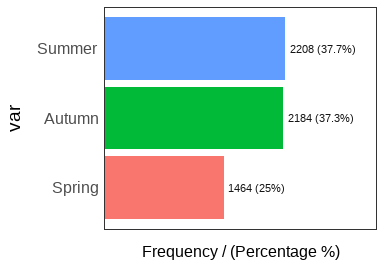
\includegraphics[width=1\linewidth]{barplot_seasons} 

}

\caption{\label{fig:fig1}Histograma de Seasons.}\label{fig:fig1}
\end{figure}

\newpage
\subsection{Análisis de la variable Bicicletas Rentadas Rented Bike Count}

Análisis de una variable tipo numérica (tabla de frecuencias, histograma
de frecuencias y curva de densidad) y análisis de normalidad (Q-Q plot y
prueba de normalidad)

\begin{table}

\caption{\label{tab:tab2}\label{tab:tab2}Tabla de frecuencias de Bicicletas Rentadas Rented Bike Count.}
\centering
\begin{tabular}[t]{l|l|r|r|r|r}
\hline
variables & levels & N & freq & ratio & rank\\
\hline
Rented\_Bike\_Count & (140,160] & 641 & 91 & 14.20 & 1\\
\hline
Rented\_Bike\_Count & (20,40] & 641 & 87 & 13.57 & 2\\
\hline
Rented\_Bike\_Count & (160,180] & 641 & 82 & 12.79 & 3\\
\hline
Rented\_Bike\_Count & (0,20] & 641 & 80 & 12.48 & 4\\
\hline
Rented\_Bike\_Count & (120,140] & 641 & 75 & 11.70 & 5\\
\hline
Rented\_Bike\_Count & (40,60] & 641 & 72 & 11.23 & 6\\
\hline
Rented\_Bike\_Count & (60,80] & 641 & 56 & 8.74 & 7\\
\hline
Rented\_Bike\_Count & (100,120] & 641 & 54 & 8.42 & 8\\
\hline
Rented\_Bike\_Count & (80,100] & 641 & 44 & 6.86 & 9\\
\hline
\end{tabular}
\end{table}

\begin{figure}[H]

{\centering 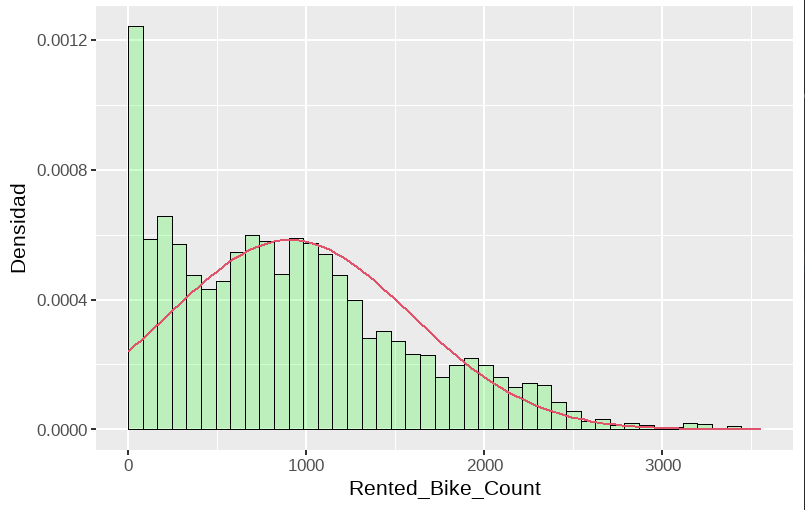
\includegraphics[width=1\linewidth]{frec_density} 

}

\caption{\label{fig:fig3}Histograma con curva de densidad de Bicicletas Rentadas Rented Bike Count.}\label{fig:fig3}
\end{figure}
\begin{figure}[H]

{\centering 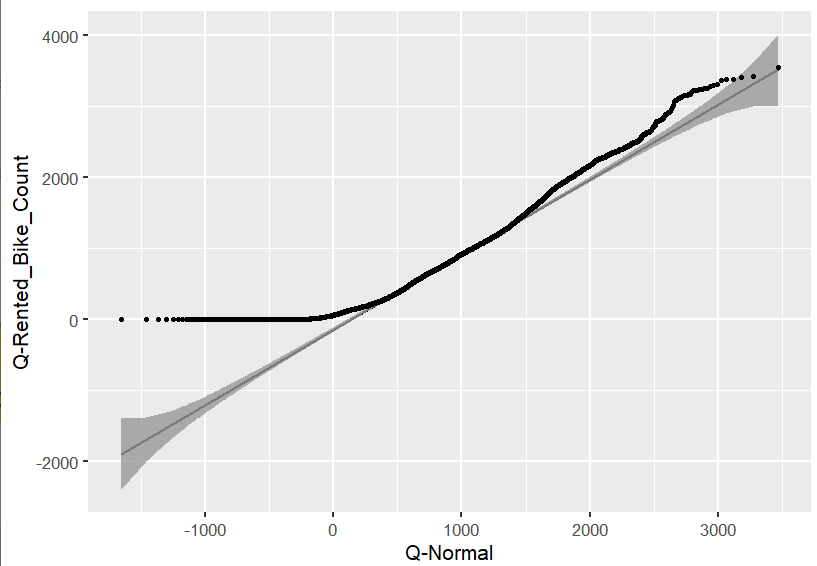
\includegraphics[width=1\linewidth]{qq} 

}

\caption{\label{fig:fig4}Q-Q plot de Bicicletas Rentadas Rented Bike Count.}\label{fig:fig4}
\end{figure}

\newpage
\subsection{Valores Atípicos}

Identificación de valores atípicos (boxplot variable numérica (2.3),
boxplot relación variable numérica (2.3) con variable entera o
categórica (2.2)

\begin{figure}[H]

{\centering 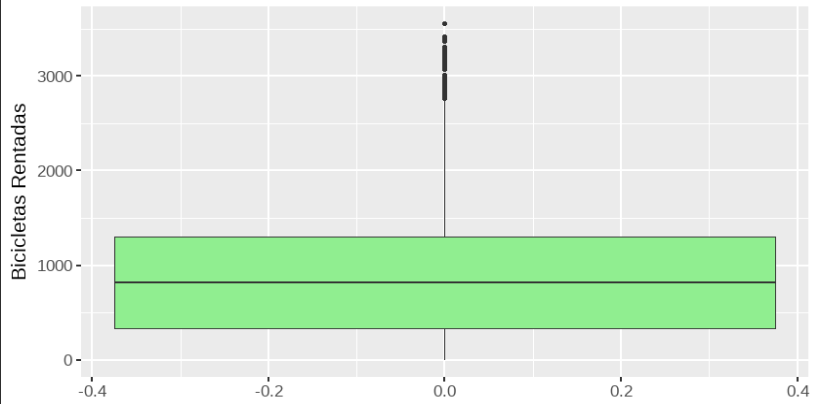
\includegraphics[width=1\linewidth]{datos_atypical} 

}

\caption{\label{fig:fig5}Datos Atípicos de Bicicletas Rentadas Rented Bike Count. }\label{fig:fig5}
\end{figure}
\begin{figure}[H]

{\centering 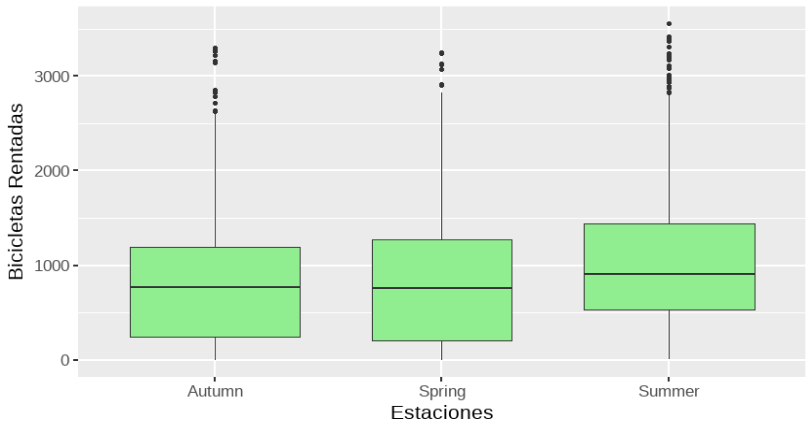
\includegraphics[width=1\linewidth]{boxplot_seasons} 

}

\caption{\label{fig:fig6}Boxplot de la variable Seasons. }\label{fig:fig6}
\end{figure}
\newpage
\subsection{Datos Faltantes}

Determinar proporción de datos faltantes

\begin{figure}[H]

{\centering 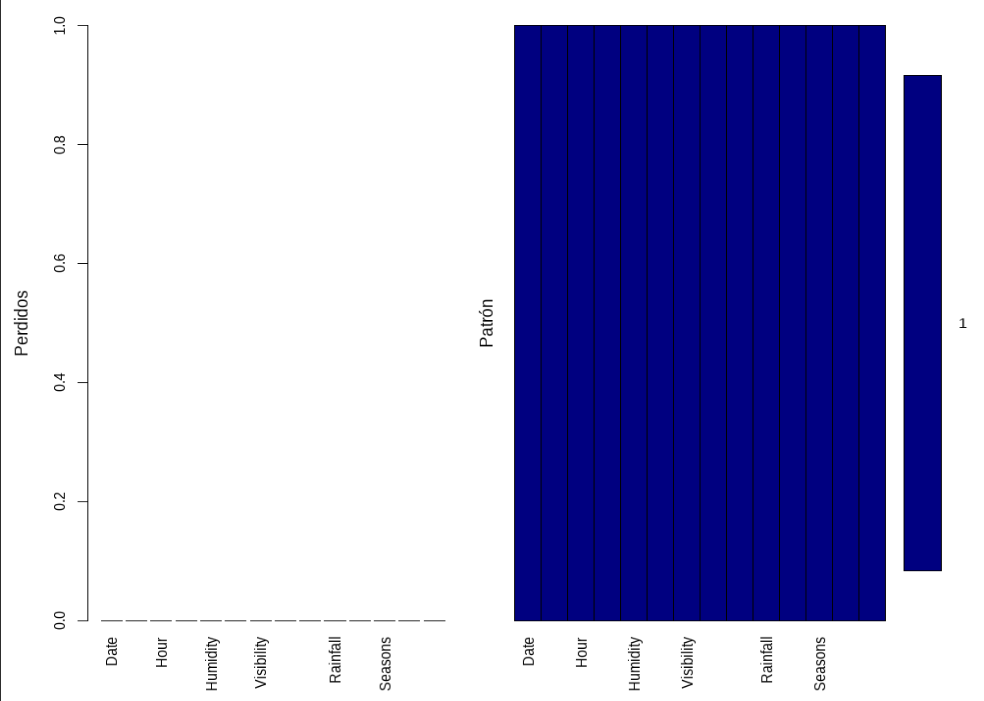
\includegraphics[width=1\linewidth]{missing_data} 

}

\caption{\label{fig:fig7}Gráfico de Datos faltantes.}\label{fig:fig7}
\end{figure}
\newpage
\subsection{Análisis de Correlación}

Análisis de correlación, representación de matriz de correlación.

\begin{figure}[H]

{\centering 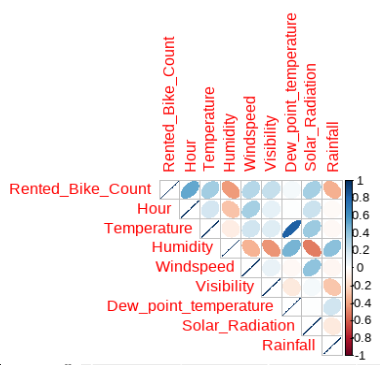
\includegraphics[width=1\linewidth]{corr} 

}

\caption{\label{fig:fig8}Matriz de Correlación.}\label{fig:fig8}
\end{figure}

\section{Conclusiones}

Resuma las principales conclusiones de cada análisis realizado como
parte del desarrollo.

\section{Referencias Bibliográficas}

Referencias Bibliográficas \{\#references .unnumbered\}

\section{Anexos}
\subsection{fig}

Ejemplo para hacer la tabla (Ver Tabla \ref{tab:tab1})

setwd(``D:\textbackslash UNAB\textbackslash MINERIA DE
DATOS\textbackslash AE1'') datos \textless-
read.csv(``rentBike\_data.csv'',sep = ``,'',header = TRUE)
diagnose\_numeric(datos) \%\textgreater\% flextable()

funModeling::freq(datos\$Seasons)

==========

\bibliography{mybibfile.bib}


\end{document}
